%----------------------------------------------------------------------------
% This version is for SN. LM has a different version of the same text.
%----------------------------------------------------------------------------

<% begin_sec("No action at a distance") %>
<% begin_sec("The Newtonian picture") %>
The Newtonian picture of the universe has particles interacting with each other by exerting
forces from a distance, and these forces are imagined to occur without any time
delay. For example, suppose that super-powerful aliens, angered when they hear disco
music in our AM radio transmissions, come to our solar system on a mission to
cleanse the universe of our aesthetic contamination. They apply a force to our
sun, causing it to go flying out of the solar system at a gazillion miles an hour. According to Newton's
laws, the gravitational force of the sun on
the earth will \emph{immediately} start dropping off. This will be detectable on earth,
and since sunlight takes eight minutes to get from the sun to the earth, the change in gravitational force
will, according to Newton, be the first way in which earthlings learn the bad news --- the sun will not
visibly start receding until a little later.
Although this scenario is fanciful, it shows
a real feature of Newton's laws: that information can be transmitted from one place in the universe to another with zero time delay,
so that transmission and reception occur at exactly the same instant.
Newton was sharp enough to realize that this required a nontrivial assumption,
which was that there was some completely objective and well-defined way of saying whether
two things \emph{happened} at exactly the same instant. He stated this assumption explicitly:
%---------------- This is the 1729 Motte translation, except for my substitution of "at a constant rate" for "equably." ------------------
``Absolute, true, and mathematical time, of itself, and from its own nature flows
at a constant rate without regard to anything external\ldots''
<% end_sec %> % Newton's instantaneous action at a distance
<% begin_sec("Time delays in forces exerted at a distance",nil,'time-delays') %>
Relativity forbids Newton's instantaneous action at a distance. For suppose that instantaneous action at a distance
existed. It would then be possible to send signals from one place in the universe to another without any time lag.
This would allow perfect synchronization of all clocks. But the Hafele-Keating experiment demonstrates that
clocks A and B that have been initially synchronized will drift out of sync
if one is in motion relative to the other.
With instantaneous transmission of signals, we could determine, without having to wait for A and B to be reunited,
which was ahead and which was behind. Since they don't need to be reunited, neither one needs to undergo any acceleration;
each clock can fix an inertial frame of reference, with a velocity vector that changes neither its direction nor its magnitude.
But this violates the principle that constant-velocity motion is relative, because each clock
can be considered to be at rest, in its own frame of reference. Since no experiment has ever detected any violation
of the relativity of motion, we conclude that instantaneous action at a distance is impossible.

Since forces can't be transmitted instantaneously, it becomes natural to imagine force-effects
spreading outward from their source like ripples on a pond, and we then have no choice but to
impute some physical reality to these ripples. We call them fields, and they have their own
independent existence. Gravity is transmitted through a field called the gravitational field.
Besides gravity, there are other fundamental fields of force such as electricity and magnetism
(ch.~\ref{ch:efield}-\ref{ch:em}). Ripples of the electric and magnetic fields
turn out to be light waves. This tells us that the speed at which electric and magnetic field
ripples spread must be $c$, and by an argument similar to the one in subsection
\ref{subsec:universal-speed} the same must hold for any other fundamental field, including
the gravitational field.

Fields don't have to wiggle; they can hold still as well. The earth's magnetic
field, for example, is nearly constant, which is why we can use it for direction-finding.
<% marg(-100) %>
<%
  fig(
    'e-field-energy-argument',
    %q{Fields carry energy.}
  )
%>
<% end_marg %>

Even empty space, then, is not perfectly featureless. It has measurable
properties. For example, we can drop a rock in order to measure the direction of the gravitational
field, or use a magnetic compass to find the direction of the magnetic field. This concept made a deep impression
on Einstein as a child. He recalled that
when he was five years old, the gift of a magnetic compass convinced him that there was ``something behind things, something deeply hidden.''
<% end_sec %> % Time delays in forces exerted at a distance
<% begin_sec("More evidence that fields of force are real: they carry energy.") %>\label{fieldenergy}
The smoking-gun argument for this strange notion of
traveling force ripples comes from the fact that they carry energy. In figure \subfigref{e-field-energy-argument}{1},
Alice and Betty hold balls A and B at some distance from one another.
These balls make a force on each other; it doesn't really matter for the sake of our argument
whether this force is gravitational, electrical, or magnetic. Let's say it's electrical, i.e., that the balls
have the kind of electrical \emph{charge} that sometimes causes your socks to cling together when they come out
of the clothes dryer. We'll say the force is repulsive, although again it doesn't really matter.

If Alice chooses to move
her ball closer to Betty's, \subfigref{e-field-energy-argument}{2}, Alice will have to do some mechanical work
against the electrical repulsion, burning off some of the calories from that
chocolate cheesecake she had at lunch.
This reduction in
her body's chemical energy is offset by a corresponding increase in the electrical interaction energy.
Not only that, but Alice feels the resistance stiffen as the balls get closer together
and the repulsion strengthens. 
She has to do a little extra work, but this is all properly accounted for in the interaction energy.

But now suppose, \subfigref{e-field-energy-argument}{3}, that Betty decides to play a trick on Alice
by tossing B far away just as Alice is getting ready to move A.
We have already established that Alice can't feel B's motion instantaneously, so the electric forces
must actually be propagated by an electric \emph{field}. Of course this experiment is
utterly impractical, but suppose for the sake of argument that the time it takes the change in the electric field
to propagate across the diagram is long enough so that Alice can complete her motion before she feels the
effect of B's disappearance. She is still getting stale information about B's position. As she moves A to the
right, she feels a repulsion, because the field in her region of space is still the field caused by
B in its \emph{old} position. She has burned some chocolate cheesecake calories, and it appears that
conservation of energy has been violated, because these calories can't be properly accounted for
by any interaction with B, which is long gone.

If we hope to preserve the law of conservation of energy, then the only possible conclusion is that
the electric field itself carries away the cheesecake energy. In fact, this example
represents an impractical method of transmitting radio waves. Alice does work on charge A, and that energy
goes into the radio waves. Even if B had never existed, the radio waves would still have carried energy,
and Alice would still have had to do work in order to create them.
<% end_sec %> % More evidence that fields of force are real: they carry energy.

\startdqs

\begin{dq}
Amy and Bill are flying on spaceships in opposite directions at such high velocities that
the relativistic effect on time's rate of flow is easily noticeable.
Motion is relative, so Amy considers herself to be at rest and Bill to be in motion. She says that
time is flowing normally for her, but Bill is slow. But Bill can say exactly the same thing.
How can they \emph{both} think the other is slow? Can they settle the disagreement by getting
on the radio and seeing whose voice is normal and whose sounds slowed down and Darth-Vadery?
\end{dq}

\includegraphics{../share/relativity/figs/spaceships-opposite-directions}

\begin{dq}
The figure shows a famous thought experiment devised by Einstein. A train is moving at
constant velocity to the right when bolts of lightning strike the ground near its front and
back. Alice, standing on the dirt at the midpoint of the flashes, observes that the light
from the two flashes arrives simultaneously, so she says the two strikes must have occurred
simultaneously. Bob, meanwhile, is sitting aboard the train, at its middle. 
He passes by Alice at the moment when Alice later figures out that the flashes happened.
Later, he receives flash 2, and then flash 1. He infers that since both flashes traveled
half the length of the train, flash 2 must have occurred first.
How can this be reconciled with Alice's belief that the flashes were simultaneous?
Explain using a graph.
\end{dq}

<%
 fig(
   'einstein-train',
   '',
   {
     'width'=>'wide',
     'sidecaption'=>true,
     'anonymous'=>true
   }
 )
%>
%-----------------------------------------------------------------------------------------------------

\begin{dq}
Resolve the following paradox by drawing a spacetime diagram (i.e., a graph of $x$ versus $t$).
Andy and Beth are in motion relative to one another at a significant fraction of $c$.
As they pass by each other, they exchange greetings, and Beth tells Andy that she is
going to blow up a stick of dynamite one hour later. One hour later by Andy's clock,
she still hasn't exploded the dynamite, and he says to himself, ``She hasn't exploded it
because of time dilation. It's only been 40 minutes for her.''
He now accelerates suddenly so that he's moving at the same velocity as Beth. 
The time dilation no longer exists. If he looks again, does he suddenly see the flash from
the explosion? How can this be? Would he see her go through 20 minutes of her life in fast-motion?
\end{dq}

\begin{dq}
Use a graph to resolve the following relativity paradox.
Relativity says that in one frame of reference, event A could happen before event B, but in someone else's
frame B would come before A. How can this be? Obviously the two people could meet up at A and talk
as they cruised past each other. Wouldn't they have to
agree on whether B had already happened?
\end{dq}

<% marg(200) %>
<%
  fig(
    'dq-pole-paradox',
    %q{Discussion question \ref{dq:pole-paradox}.}
  )
%>
<% end_marg %>

\begin{dq}\label{dq:pole-paradox}
The rod in the figure is perfectly rigid. At event A, the hammer strikes one end of the rod.
At event B, the other end moves. Since the rod is perfectly rigid, it can't compress, so A
and B are simultaneous. In frame 2, B happens before A. Did the motion at the right end \emph{cause}
the person on the left to decide to pick up the hammer and use it?
\end{dq}


<% end_sec %> % No action at a distance
